\section{Experiments on image classifiers}
\label{sec:image-experiments}

We tested the support condition on raw parameterizations produced by
minibatch optimization. These experiments do not sample from the Bayesian
prior or posterior. In particular, a trained network's test accuracy does
not verify the posterior generalization theorem.

\paragraph{Tasks and optimization.}
The data are the official MNIST and Fashion-MNIST training and test sets.
The two-class tasks use all MNIST digits 3 and 8, and all Fashion-MNIST
classes 0 and 6. A harder task uses all $60{,}000$ MNIST training images
and $10{,}000$ test images with an even-versus-odd label. The main
architecture is a plain tanh network with width $128$, $256$, or $512$,
hidden depth $4$, $16$, or $32$, a first-layer bias, and a scalar linear
readout. There are no later hidden biases and no residual connections.
Training uses logistic loss and actual shuffled minibatches of size $128$.
Vanilla stochastic gradient descent (SGD) and Adam are distinguished;
a small exploratory rectified linear unit (ReLU) cohort uses momentum
SGD and lies outside the tanh theorem.

Every cohort has a timestamped protocol fixed before that cohort's
training. Later cohorts were motivated by earlier observations, so the
whole research sequence is exploratory. All runs, including failed fits
and collapsed classifiers, are retained. We use the final prescribed
checkpoint and never rescale its readout. Unless separately declared,
training lasts $60$ epochs. The two depth-$32$ MNIST SGD seeds also have
separately recorded continuations for $180$ further epochs, at a fixed
lower learning rate; both original models remain in the data.
Four later SGD runs probe depths $64$ and $128$ at width $128$, with
fixed orthogonal initialization gains $1$ and $1.1$.
All four also receive separately declared $180$-epoch lower-rate
continuations; the original fixed-budget runs remain in the record.

Continuous pixels are mapped to $[-1,1]$ in float32; Boolean pixels use
threshold $128$. Final metrics and ordinary numerical audits cast those
same input values and saved weights to float64. Thus auditing does not
change the represented input. These are small fully connected image
models, rather than modern convolutional networks or transformers.

\paragraph{Eligibility and calibration.}
For every model we separately record whether \emph{all} training signed
outputs exceed $1/2$. High accuracy alone does not meet this likelihood
condition. The primary score is clipped at $\pm1/2$, the allowed score
change is $1/16$, and the radius constants are
\[
 c\in\{0.001,0.003,0.01,0.03,0.0625\}.
\]
The primary constant is $0.001$; the rest are a fixed calibration study.
The cap $1$ is an additional recorded comparison. Neither radius nor
readout scale is adjusted to make an individual model pass.

\IfFileExists{experiment/results-tables.tex}{\begin{table}[t]
\centering\small
\begin{tabular}{lrrr}
\toprule
Cohort & Runs & All train margins $>1/2$ & Test accuracy (\%) \\
\midrule
Initial continuous images & 24 & 3 & 49.95--99.55 \\
Initial Boolean images & 8 & 1 & 49.95--99.19 \\
Initial width-$256$ extension & 4 & 1 & 49.95--99.29 \\
Width-$512$ extension & 4 & 3 & 87.10--99.50 \\
All MNIST, even versus odd & 4 & 4 & 98.92--99.03 \\
ReLU comparisons & 4 & 3 & 86.90--99.13 \\
Spectral-projection intervention & 4 & 0 & 86.20--98.95 \\
Additional matched reference & 1 & 0 & 87.15 \\
Projected-SGD continuation & 1 & 0 & 98.83 \\
Depth-$32$ SGD continuations & 2 & 1 & 99.14--99.24 \\
Depth-$64/128$ extension & 4 & 0 & 98.79--98.99 \\
Depth-$64/128$ continuations & 4 & 0 & 98.74--98.94 \\
Enumerated Boolean domains & 6 & 6 & 92.86--100.00 \\
\midrule
Total & 70 & 22 & \\
\bottomrule
\end{tabular}
\caption{Every declared training run is retained. Accuracy ranges are descriptive extrema over the specified cohort, not confidence intervals. Continuations are additional parameterizations of retained original runs. Training-margin eligibility is separate from robustness.}
\label{tab:training-cohorts}
\end{table}
\begin{table}[t]
\centering\small
\begin{tabular}{lrrrr}
\toprule
 & \multicolumn{2}{c}{Test accuracy (\%)} & \multicolumn{2}{c}{Minimum train margin} \\
Task, depth & SGD & Projected & SGD & Projected \\
\midrule
MNIST even/odd, $H=4$ & 98.94 & 98.95 & 2.69 & -3.59 \\
MNIST even/odd, $H=16$ & 98.92 & 98.87 & 4.49 & -1.66 \\
Fashion 0/6, $H=4$ & 87.15 & 87.10 & -4.96 & -5.44 \\
Fashion 0/6, $H=16$ & 86.85 & 86.20 & -3.41 & -4.10 \\
\bottomrule
\end{tabular}
\caption{Matched spectral-projection intervention. The models share initialization and minibatch order, and receive the same gradient-step budget. Raw readouts are not rescaled.}
\label{tab:projected-training}
\end{table}
}{}

The final collection contains $70$ parameterizations: $60$ tanh image
models, four ReLU comparisons, and six Boolean-domain models.
Every training margin exceeds $1/2$ for $13$, three, and six of these,
respectively, for a total of $22$. These counts include every prescribed
failed fit and every separately retained continuation.

\paragraph{Pointwise audit and its limits.}
For each tanh image model the prescribed audit uses uniformly sampled held-out
images, the $16$ held-out images with smallest absolute clean output,
and independent uniform Boolean-cube probes. The second group is
deliberately concentrated near the decision boundary. At width $512$,
the uniform positive-certificate budget is reduced to the first $32$
of the same prescribed $128$ points. Figure~\ref{fig:empirical-coverage}
uses common per-model denominators: $32$ uniform images, $16$ boundary
images, and $32$ Boolean probes at every radius. Missing or inconclusive
certificates remain unresolved. A companion file applies exactly the
same display rules to training-margin-eligible models only.

The positive audit propagates finite reachable-state bounds and
saturation-aware tanh remainder bounds. Its ordinary pointwise results
use float64 evaluations of sufficient inequalities. Attacks optimize
both raw-output directions over simultaneous perturbations of every
hidden layer and the scalar output, with two starts and $100$ projected
gradient steps per direction. The main attack subset is the first $16$
points of each group; points without an attack search are still certified
only when a positive bound succeeds. All observed violating tuples are saved
and re-evaluated strictly inside the prescribed budget. Selected positive
and negative results receive independent exact-rational or outward
interval verification, as described separately. An unsuccessful attack
is not a positive certificate, and an unsuccessful certificate is not
a counterexample. Pooled input/model counts reuse data and are not
independent statistical observations.

Among the $13$ training-margin-eligible tanh image models, the primary
radius receives sufficient float64 certificates on all $1{,}184$
uniformly held-out, $208$ boundary held-out, and $832$ random Boolean
input/model pairs in the prescribed positive-certificate subsets.
At $c=0.01$, the corresponding counts are $1{,}181$, $150$, and $820$.
These finite sampled successes coexist with the separately targeted
global counterexamples below. An independent audit compares all
$28{,}800$ matched attack/certificate evaluations across the $60$ tanh
image models; none exceeds its sufficient bound beyond $10^{-8}$.

\begin{figure}[t]
\centering
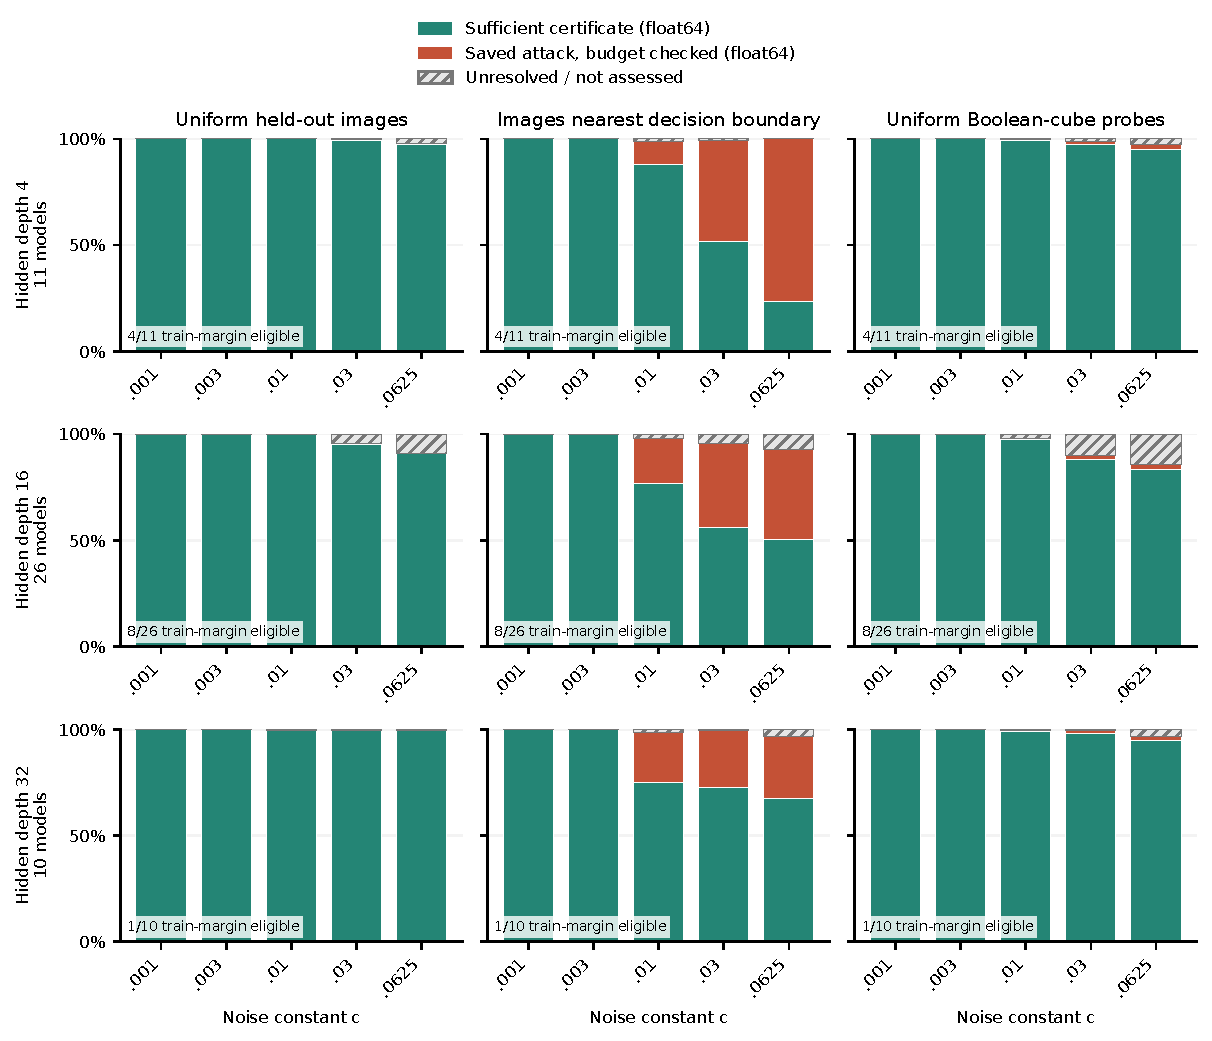
\includegraphics[width=.99\textwidth]{figures/certificate-coverage.pdf}
\caption{Fixed-subset audit of all depth-$4/16/32$ unconstrained tanh runs, including
failed training fits. Green denotes a sufficient finite-radius
certificate evaluated in float64; red denotes an explicit saved attack
that passes a float64 budget and score recheck; hatched gray denotes an
unresolved or unassessed point. Selected exact verifications are reported
separately. The same points and denominators are used at every radius.
Boundary images and uniform Boolean probes have different sampling
interpretations from uniformly selected test images.}
\label{fig:empirical-coverage}
\end{figure}

\paragraph{A same-model positive and negative result.}
The Boolean-input MNIST model \texttt{029} has hidden depth $16$, width
$128$, was trained by vanilla SGD, and has minimum training signed
output above $4.23$ and test accuracy $99.19\%$. Its raw output has a
global all-real-input certificate at $c=0.001$. At $c=0.01$, exact-budget
checks and outward interval arithmetic verify clipped-score violations
on both a held-out Boolean image and a uniform Boolean probe. The score
changes exceed $0.0845$ and $0.0855$, respectively. In both attacks every
disturbed hidden state remains in $[-1,1]$. Thus the calibration constant
matters even for a fitted classifier, and the larger-radius failures
are not caused by allowing hidden states outside the activation range.

The full-MNIST even-versus-odd model \texttt{104}, with hidden depth $4$
and width $256$, fits every training margin above $2.68$, reaches
$98.94\%$ test accuracy, and has an exact-rational global certificate
at $c=0.003$: its raw output changes by at most $0.03230<1/16$.
This certificate covers every real input, not merely the recorded
images. The statement concerns its trained parameterization; it does
not identify its training process with Bayesian inference.

The matched-task depth-$16$, width-$256$ model \texttt{105} illustrates
the limitation of a universal support claim. Exact integer/rational
verification puts all $60{,}000$ training signed margins above $4.48157$.
Certified clean-output intervals give $9{,}892$ correct predictions among
the $10{,}000$ test labels, confirming $98.92\%$ accuracy. Yet it has a rigorously
verified violation already at the primary constant
$c=0.001$. A synthesized 8-bit image with mean ink about $0.172$ and
$64.2\%$ black pixels has clean output approximately $-0.00163$ and
perturbed output $-0.15496$, giving clipped-score change above $0.1533$.
Every disturbed hidden state remains in $[-1,1]$. This is a constructed
off-distribution image, not a held-out natural image, and its encoding
into Boolean pixel bits is discussed separately. Thus fitting every
training margin does not by itself enforce the proposed global
condition.

A later, separately declared search addresses the objection that the
first witness starts near the decision boundary. On another synthetic
8-bit input, the same model has clean output in
$[0.53934,0.53935]$, above the training margin. A hidden-only disturbance
at $c=0.001$ lowers it to $[0.38661,0.38662]$, below $7/16$.
The scalar output disturbance is exactly zero, and every disturbed
hidden coordinate remains inside $[-1,1]$. Exact budget and outward
interval checks establish this for both rational pixel normalization
and the original float32 preprocessing. Thus the global failure also
affects a confident positive output and violates the training-level
implication~\eqref{eq:transport-training-level} of the optional two-margin
transport condition (Appendix~\ref{sec:two-margin-transport}); no true label is assigned to this
constructed image.

This failure is sharply separated from the observed image distribution.
A separately declared follow-up checked \emph{every} official held-out
image for selected models. For model \texttt{105}, all $10{,}000$ images
receive a sufficient pointwise certificate at both $c=0.001$ and
$c=0.003$. At the latter constant, $9{,}960$ pass by combining the global
raw-output bound with clipping, and the remaining $40$ pass using local
finite-radius bounds. Both original depth-$32$ MNIST SGD seeds similarly
certify all $1{,}984$ test images at both constants, despite their failed
training-margin fits. These initial whole-pool sweeps evaluate sufficient
inequalities in float64 on a finite held-out set; they do not cover every
natural image or the whole input cube.
Across all six prescribed follow-up models
(\texttt{005}, \texttt{008}, \texttt{009}, \texttt{029}, \texttt{105}, and
\texttt{107}), all $27{,}936$ held-out input/model pairs are certified
at both constants. Eleven initially unresolved points for model
\texttt{107} at $c=0.003$ were subsequently certified by stronger
finite-radius enclosures; that refinement history is retained.

Model \texttt{105} subsequently receives an exact upgrade at the primary
constant $c=0.001$: exact integer/rational arithmetic and outward
interval bounds certify every one of its $10{,}000$ official test inputs,
using their original float32-normalized values. A global bound covers
$9{,}988$ inputs and local bounds cover the remaining $12$, with maximum
certified clipped-score change below $0.017653<1/16$.
This quantifies over every allowed simultaneous disturbance at each of
those inputs. It does not certify unknown images or the population
distribution. The result at $c=0.003$ and the other models' whole-pool
results retain their float64 qualification.
The same exact method also verifies the training-margin statement above
and clipped-score stability at all $60{,}000$ training inputs at
$c=0.001$. Thus this model has verified likelihood eligibility and
verified stability on both official data sets while still failing the
global input-domain condition.

\paragraph{An explicit spectral-norm intervention.}
Four further vanilla-SGD runs project every hidden-to-hidden matrix
to operator norm at most $0.99$ after each epoch, including after the
final update. The first layer and readout are untouched. Each has a
matched unconstrained run with the same initialization, minibatch order,
data, number of gradient steps, and learning-rate schedule. The
nonexpansive certificate then guarantees score stability up to
$c=1/16$ when the saved internal norms are verified below one.
This is an intervention in training, rather than evidence that ordinary
SGD spontaneously enforces the condition. Its accuracy and training
margin cost must be assessed alongside the guaranteed stability.
The matched MNIST test accuracies change from $98.94\%$ to $98.95\%$
at depth $4$, and from $98.92\%$ to $98.87\%$ at depth $16$.
Fashion test accuracy decreases by $0.05$ and $0.65$ percentage points,
respectively. All four projected runs retain training errors and hence
fail the hard training-margin likelihood. They demonstrate useful
classification under an enforced support restriction, not fitted
examples under that likelihood.
The separately declared continuation for $240$ additional epochs of the depth-$16$
full-MNIST projected run still has $154$ training errors, compared with
$169$ initially, and test accuracy $98.83\%$. Thus the fixed longer
optimization budget does not resolve the training-likelihood failure.
All five projected parameterizations nevertheless have exact-rational
global certificates at $c=1/16$, including the continued model, whose
uniform raw-output variation bound is below $0.058087$.

\paragraph{A polynomial-depth calibration variant.}
After observing the fixed-radius failures, we also screened the
explicitly exploratory choice $c_H=0.001/H$. This weakens the radius by
one additional power of depth; a theorem polynomial in $c+c^{-1}$
continues to have polynomial depth dependence under this substitution.
For the same model \texttt{105}, exact-rational operator bounds certify
global raw-output variation at most $0.023658$ at $c_H=1/16000$, so
it passes this weaker condition on every real input. This does not
undo its failure at the original fixed constant. The larger-depth
cohort tests this variant further, without inferring an asymptotic
law from finitely many trained networks.
The fitted depth-$32$ continuation \texttt{301} yields the same
distinction: an interval-verified primary-radius violation coexists
with an exact global raw-variation bound below $0.017821$ at
$c_H=1/32000$. Its minimum training margin is $2.41066$ and test
accuracy is $99.244\%$; the other prescribed continuation still has
three training errors.

\IfFileExists{figures/projected-sgd-comparison.pdf}{
\begin{figure}[t]
\centering
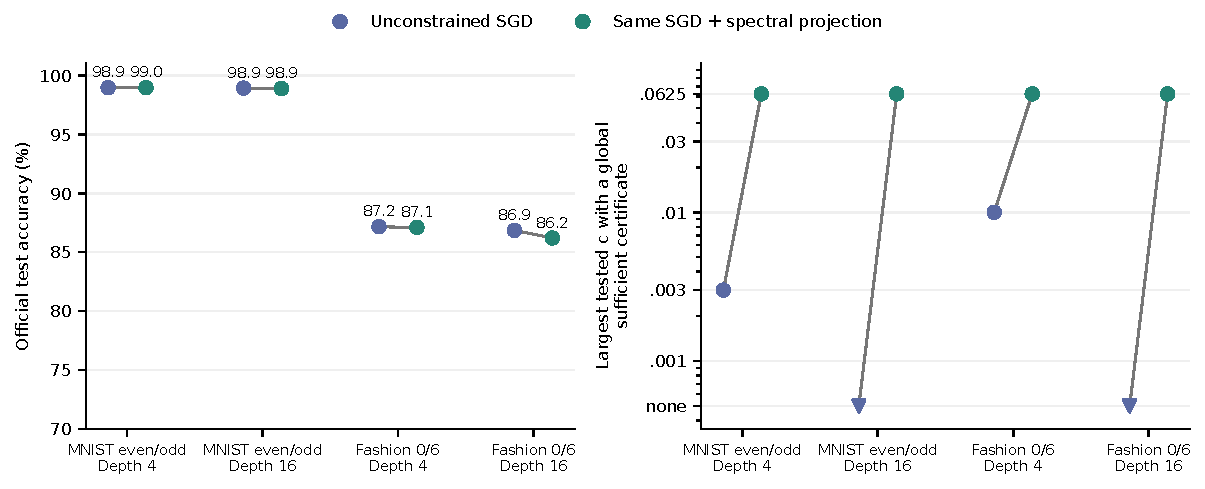
\includegraphics[width=.99\textwidth]{figures/projected-sgd-comparison.pdf}
\caption{Matched vanilla-SGD comparison with and without a spectral
projection after each epoch. The right panel gives the largest tested
radius constant with a global sufficient certificate, a lower bound
on stability rather than an estimate of the largest valid radius.
Training-margin eligibility is reported separately from accuracy.}
\label{fig:projected-comparison}
\end{figure}}{}

\paragraph{Reduced-precision diagnostic.}
We additionally round hidden activations to IEEE float16 or bfloat16,
leaving weights fixed, on the official test set. Hidden-only rounding
and hidden-plus-output rounding are separate modes. The realized joint
noise norm is recorded and compared with each calibrated radius. This
is one deterministic perturbation map, not a test of every allowed
perturbation and not a worst-case certificate. In particular, successful
rounding can occur even when its realized noise lies outside the
certified ball.
The smallest calibrated ball should not be equated with
ordinary low-precision arithmetic: the realized rounding budgets can
exceed it even when the classifier's clipped score barely changes.
The complete diagnostic reports both the score changes and the actual
noise-budget coverage.

\IfFileExists{experiment/quantization-results-table.tex}{\begin{table}[t]
\centering\small
\begin{tabular}{llrrrr}
\toprule
Format & Rounded values & Sign flips & Score changes $>1/16$ & $c=.001$ & $c=.0625$ \\
\midrule
float16 & Hidden & 1 & 0 & 0.00\% & 87.52\% \\
float16 & Hidden and output & 1 & 0 & 0.00\% & 32.28\% \\
bfloat16 & Hidden & 19 & 54 & 0.00\% & 1.22\% \\
bfloat16 & Hidden and output & 19 & 53 & 0.00\% & 0.05\% \\
\bottomrule
\end{tabular}
\caption{Deterministic activation-rounding diagnostic on 175,520 held-out input/model pairs across 60 tanh image models. The last two columns give the fraction whose realized joint noise lies inside the corresponding calibrated ball. The clipped score has cap $1/2$. Failures to fit the training likelihood are retained; no adversarial or distribution-wide claim follows from this fixed rounding map.}
\label{tab:quantization}
\end{table}
}{}

\paragraph{Exhaustive Boolean audit.}
Six additional networks use the exact domain $\{-1,1\}^9$, with target
either majority of the nine bits or majority of the three majorities
on disjoint groups of three. A fixed permutation selects $400$ training
and $112$ held-out inputs. Width is $64$, hidden depths are $4$, $16$,
and $64$, and every model receives the same prescribed $500$-epoch SGD
schedule. These models are reported separately from the image cohort.
The audit enumerates all $512$ inputs at the original five radius
constants and at $c_H=0.001/H$. Thus successful coverage concerns the
entire Boolean target domain, even when a sufficient bound uniform over
all real inputs is inconclusive. Domain coverage is exhaustive, but
the arithmetic is still float64 unless separately verified exactly.
All six runs fit the training margin empirically. The initial exhaustive
audit certifies all vertices at $c=0.001$ for five models, and $511$ of
$512$ for the remaining depth-$64$ recursive-majority model; all six
pass on every vertex at $c_H$. A separately recorded stronger bound
resolves the last vertex, enclosing its noisy raw output in
$[-2.45149,-2.36141]$ and hence giving zero clipped-score change.
Thus all six ultimately pass on the entire Boolean domain at the
primary constant. These finite examples test the support condition, not an
empirical sample-complexity law.

The predeclared first exact verification selected depth-$4$ majority
model \texttt{500} at $c=0.03$. Exact interval arithmetic verifies all
$400$ training signed margins above $1/2$ and all $512$ clean absolute
outputs above $4.72037$. Combined with an exact uniform raw-output
variation bound below $0.162903$, this proves that every clipped score
is constant throughout the allowed noise ball on the entire Boolean
domain. The raw variation bound exceeds $1/16$, so this certificate
uses clipping rather than merely a small raw-output bound; it does not
show that the network violates the raw-output stability condition.

A deeper exact positive is model \texttt{504}, the depth-$64$ majority
network. All $400$ training margins are interval-verified, and the
network correctly labels $511$ of the $512$ Boolean vertices. At the
primary constant $c=0.001$, an exact finite partition and reachable-tube
calculation proves zero clipped-score change on every vertex for every
allowed simultaneous perturbation. The scalar global raw-output bound
is approximately $13.4145$ and is insufficient on its own. Thus this
is a fitted deep SGD example satisfying the actual finite-domain
support condition, certified using the states reached by its inputs.
The depth-$64$ recursive-majority model \texttt{505} also receives an
exact all-domain certificate at $c=0.001$, combining $511$ reachable-tube
cases with an exact covariance calculation for the remaining vertex.
Every training margin is interval-verified above $7.47388$; it correctly
labels $504$ of the $512$ vertices. Both deep examples thus satisfy the
support condition without requiring perfect generalization.

\IfFileExists{experiment/boolean-results-table.tex}{\begin{table}[t]
\centering\small
\begin{tabular}{lrrrrrr}
\toprule
Target & $H$ & Min. margin & Test acc. & $c=.001$ & $c=.001/H$ & All-input $c_*$ \\
\midrule
Majority9 & 4 & 4.99 & 100.00\% & 512/512 & 512/512 & 0.0625 \\
Majority9 & 16 & 6.94 & 100.00\% & 512/512 & 512/512 & 0.0625 \\
Recursive majority & 4 & 4.04 & 100.00\% & 512/512 & 512/512 & 0.0625 \\
Recursive majority & 16 & 6.56 & 96.43\% & 512/512 & 512/512 & 0.03 \\
Majority9 & 64 & 7.61 & 99.11\% & 512/512 & 512/512 & 0.001 \\
Recursive majority & 64 & 7.47 & 92.86\% & 512/512 & 512/512 & 0.001 \\
\bottomrule
\end{tabular}
\caption{Exact finite Boolean domains, with float64 evaluation of sufficient finite-radius inequalities. Certified counts cover all $512$ inputs; $c_*$ is the largest original-grid constant for which every input passes, a lower bound on the valid radius rather than an estimate of its maximum. The minimum margin is over the $400$ training inputs. One initially unresolved vertex at $c=.001$ receives a separately recorded stronger certificate. A failed sufficient certificate remains unresolved; it is not a counterexample.}
\label{tab:boolean-fullcube}
\end{table}
}{}

The experiment directory preserves protocols, raw weights, dataset
hashes, per-example outputs, failed fits, all saved attack witnesses,
certificate records, and plotting code. Exact proofs, pointwise
numerical evidence, and empirical training outcomes have distinct
qualifications throughout.
